%----------------------------------------------------------------------------
\chapter{\osszefoglalas}
%----------------------------------------------------------------------------

\section{Eredmények}

A diploma dolgozatom elején kitűzött feladatokat maradéktalanul sikerült elvégeznem. Sikeresen elkészítettem egy telemanipulátort, aminek a jelfeldolgozó rendszerével kinematikai számításokat alkalmazva, vezérlési utasításokat tudtam adni egy szimulációs környezetben létrehozott, és egy valós kollaboratív robotnak. Mindkét esetben a vezérlés stabilan fennállt, így folyamatosan tudtam vezérelni a robot és megfigyelni a jelenlegi összeállításom sajátosságait.

\begin{figure}[!ht]
\centering
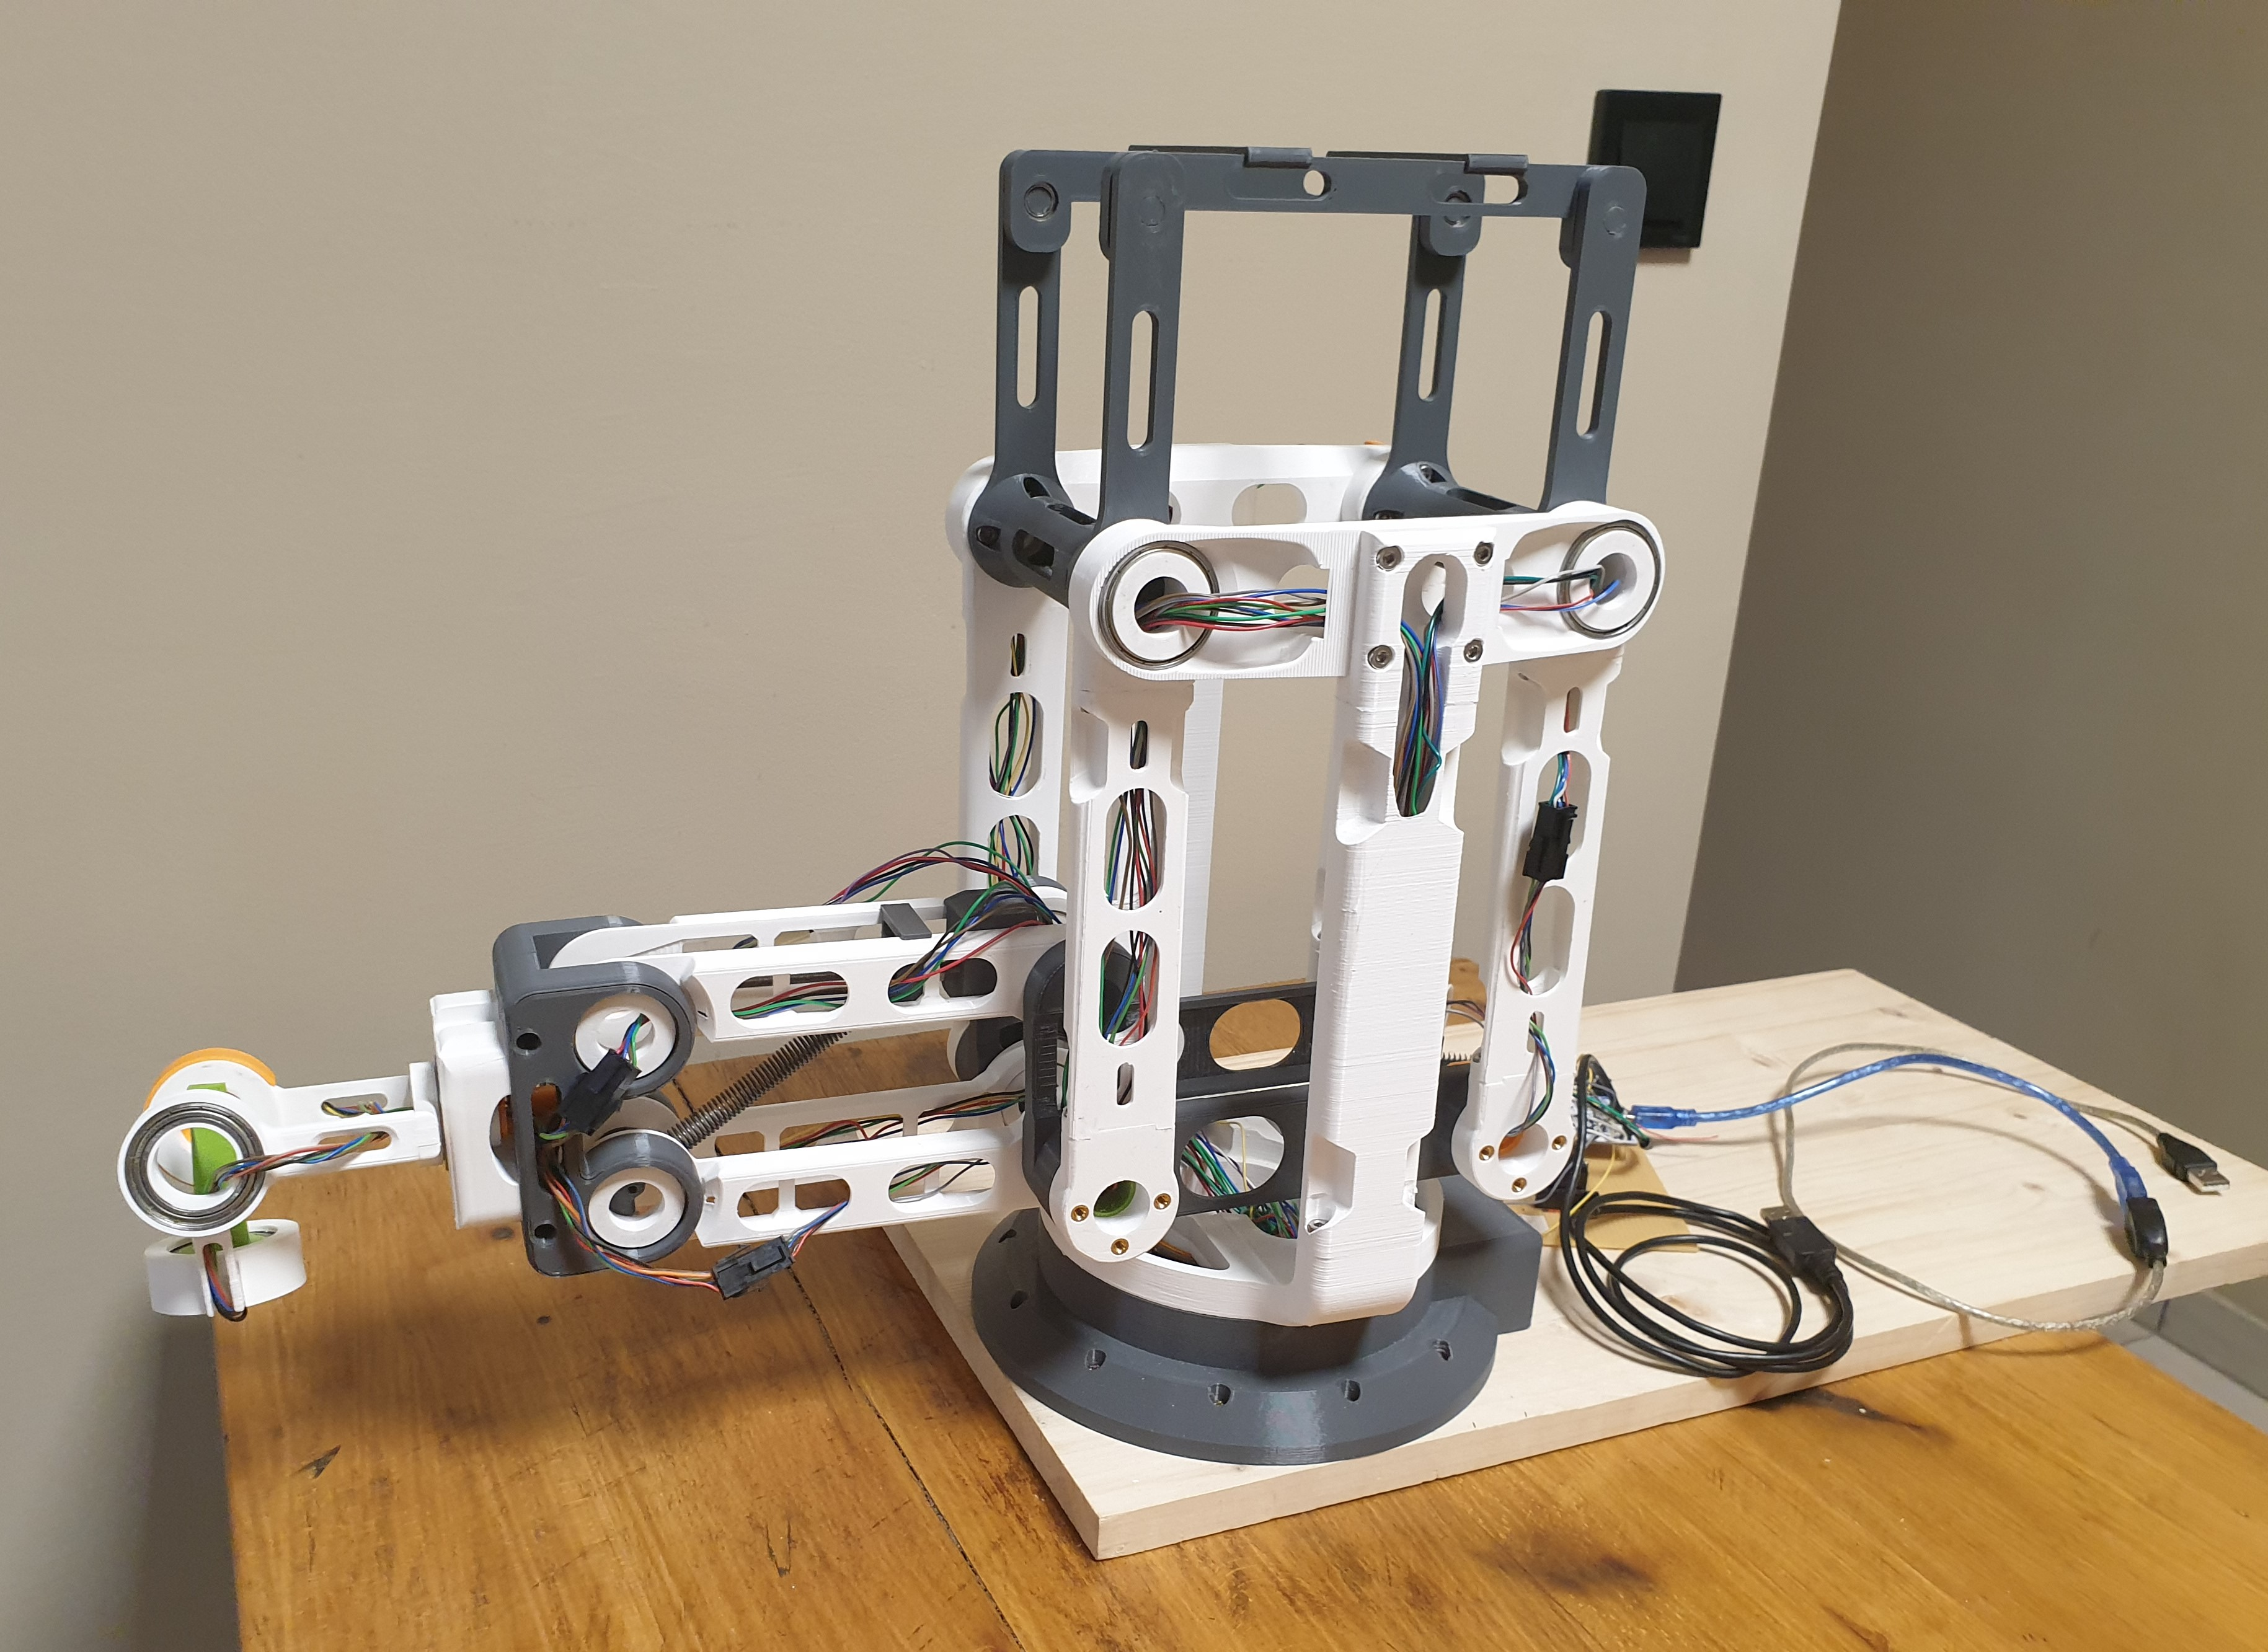
\includegraphics[width=100mm, keepaspectratio]{figures/Szumma/Keszeszkoz}
\caption{Diplomamunkám végeredménye}
\label{fig:Diploma_ending}
\end{figure}

Tanulmányaim alatt elsajátított készségek lehetővé tették, hogy a telemanipulátorral kezdeti fizikai világból gyűjtsek szenzorokkal információt a operátor mozgatási szándékáról. Ezt egy zárt szoftveres környezetben robot vezérlési paranccsá alakítsam és ezt továbbítva fizikai világban ezt a robot megvalósítsa ezt.


\section{Tanulságok és tovább fejlesztési irány} 

A telemanipulátor gyakorlatilag minden egyes elemén, amiről a diplomamunkában beszámoltam van lehetőség továbbfejlesztésre.

A telemanipulátor karjainak kialakítását a negyedik és ötödik csukló között át lehet alakítani annak érdekében, hogy a mozgás tartományt ki lehessen használni rugós mechanizmus ellenére is.

A szoftveres rendszerben a szöghibák egységnyi csökkentése vagy egy zajszűrő rendszer illesztése lehetne megfelelő irány, mivel az eredmények alapján nagyon nagy mértékben befolyásolja a szenzorok zaja a robot stabilitását. A további részekben a kontroller kialakítása funkcionális tekintetben is nagy mértékben javítható. Az egész kontroller pálya tervező motorja, illetve a ROS egyes verziójáról a kettesre átállni lehet az egyik legfontosabb cél. Ezzel célkitűzéssel  számtalan új lehetőség kerülne fel a látószögbe és kezdődhetne meg tesztelésük. A szoftveres rendszer legnagyobb és elég általánosnak mondható tanulsága talán, hogy számtalan megoldási lehetőség közül lehet választani és iteratívan tapasztalat szerzéssel lehet csak előre haladni.

Számomra a legnagyobb célkitűzés az lenne, ha egy más gyártó által elérhető robotot is megtudnék vele mozgatni. Erre nem tértem ki a dolgozatomban, de egy KUKA robot mozgatása lehetne a következő mérföld kő, mivel sokkal zártabb vezérlő rendszere van, sokkal kevésbé egyszerűsíthető és megköveteli a valósidejű lefutást.

Egy jövőbe mutató kiegészítés, ha mind ezek vezeték nélkül történnének. Azaz előkészítem a telemanipulátoromat a vezeték nélküli vezérelhetőségre, akár WiFi akár 5G hálózatokon keresztül.

A felsoroltak mellett számtalan módon lehet még ezt a rendszert tovább fejleszteni vagy esetleg új funkciókat hozzáilleszteni.

% Keltezés, aláírás
\vspace{1cm}

\begin{flushleft}
{Budapest, \today}
\end{flushleft}

\begin{flushright}
\emph{\authorName}
\end{flushright}

\vfill
